% \chapter{Desenvolvimento/Implementação}\label{cap:development}

% Neste capítulo é descrito o trabalho de implementação, salientando os pontos mais relevantes da mesma, dificuldades  encontradas ou soluções técnicas inovadoras desenvolvidas ou aplicadas.  Em particular, se foi usado código desenvolvido por terceiros (por exemplo, código {\it open-source}), deve ser facilmente distinguível quais as funcionalidades originais do mesmo e o que foi necessário implementar para obter as funcionalidades desejadas.


\chapter{Arquitetura do sistema}\label{cap:development}
Neste capítulo, é abordado em detalhe a arquitetura e a estrutura adotada para a construção dos componentes do sistema. É importante compreender que o sistema foi concebido como um conjunto de módulos, com cada um desempenhando funções específicas, e quando operados em conjunto, esses módulos resultam na realização dos propósitos pensados para o sistema.

O sistema é estruturado fundamentalmente em camadas distintas, o backend, o frontend, e o banco de dados.

\begin{figure}[htbp]
	\centering
	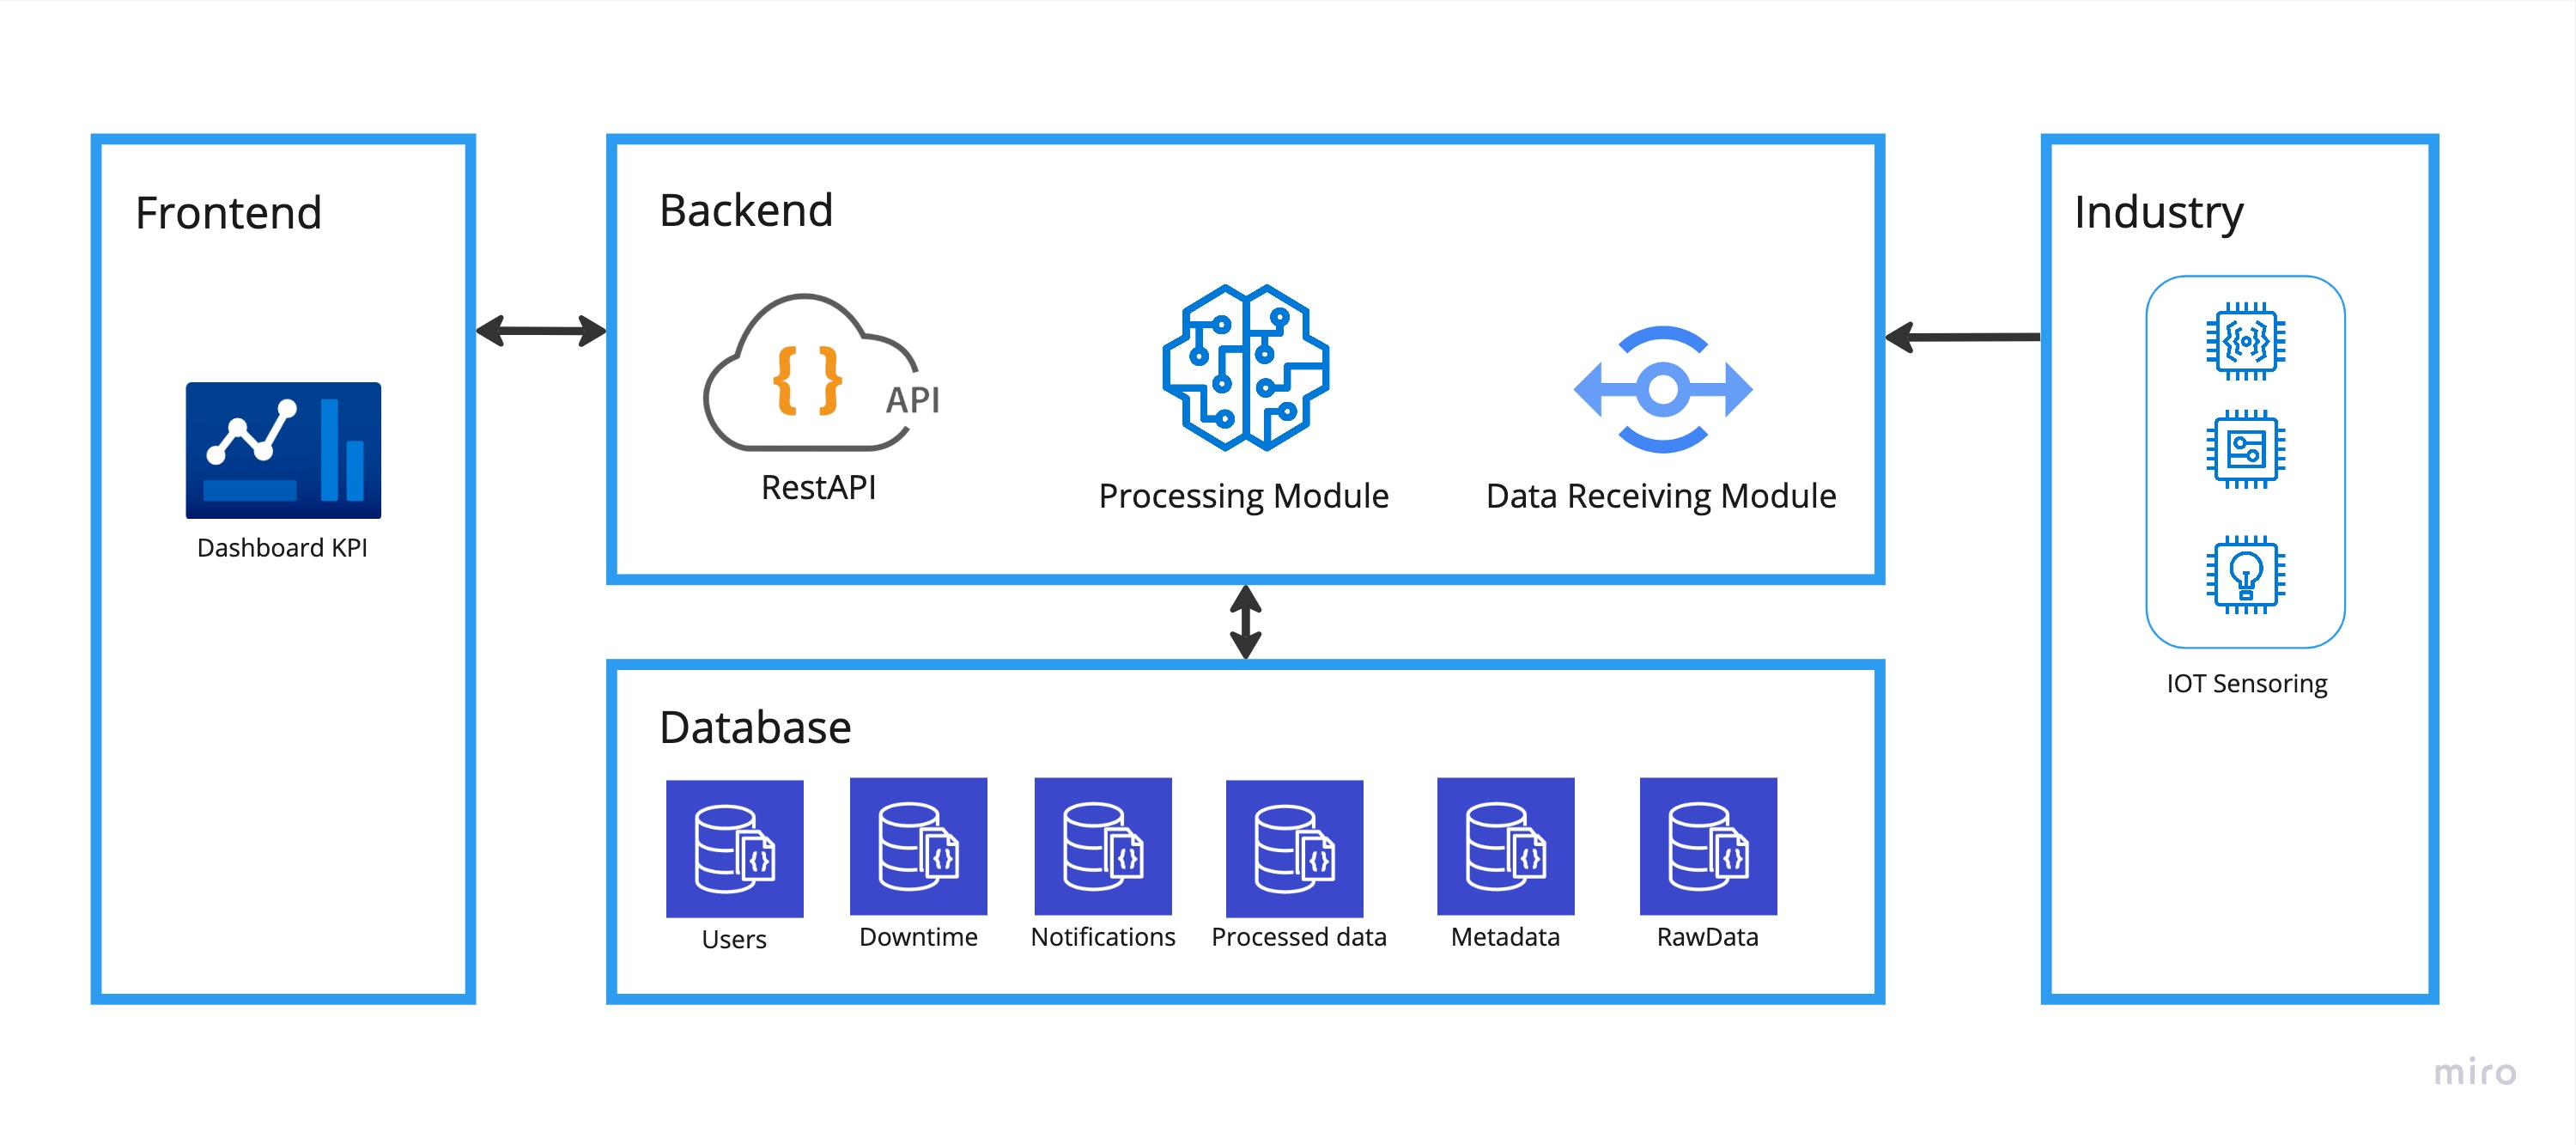
\includegraphics[width=\textwidth]{images/Architecture.jpg}
	\caption{System architecture.}
	\label{fig:systemAchitectureImage}
\end{figure}

%TODO Sigla api
O backend funciona como o núcleo do sistema. Sua principal função é a de receber os dados, processá-los conforme as regras estabelecidas nos requisitos e histórias de usuários e, armazená-los de maneira segura no banco de dados. Além das funções de armazenamento e processamento, ao backend também é atribuída a responsabilidade de disponibilizar esses dados por meio de uma interface de programação de aplicações (API), que pode ser acessada utilizando métodos HTTP. Esta API age como um intermediário entre a lógica central do sistema e as interfaces com as quais o usuário final interage, o frontend.

%TODO referencia para princípios de design e data visualization - Talvez referir a outra parte da dissertação que entra em mais detalhes
Por outro lado, o frontend é caracterizado como a interface visual que o usuário final acessa. Serve como meio pelo qual os usuários interagem com o sistema, enviando e recebendo informações. Esta camada é projetada para acessar, recuperar e apresentar os dados processados e armazenados pelo backend de uma maneira intuitiva e amigável, utilizando princípios de design e data visualization.

Como pode ser visto na figura~\ref{fig:systemAchitectureImage}, na planta industrial, onde as máquinas com os sensores se encontram, os sensores enviam os dados para o sistema, que recebe eles por meio do modulo de recebimento de dados e os armazena no banco de dados. O modulo de processamento acessa os dados armazenados para realizar a agregação, e a API gerencia o acesso ao banco de dados, disponibilizando as informações para os usuários no frontend.

Nas seções seguintes, cada um desses componentes será explorado mais profundamente, passando por suas especificidades e interações.


\section[Arquitetura do backend]{Arquitetura backend}
%TODO Sigla HTTP
Nessa seção é abordado o funcionamento do backend. Ele está dividido em três partes, o module de recebimento dos dados dos sensores, o modulo de processamento onde é feita a agregação e analise estatística dos dados, e a API que gerencia o acesso as informações por meio de requisições HTTP.

Em relação a organização dos repositórios, a API e o modulo de recebimento de dados ficam no mesmo repositório, facilitando a comunicação entre eles. Já o modulo de processamento está em um repositório a parte, sendo a sua única função sendo ler o banco de dados, processar os dados, e armazenar os resultados.

\subsection{Modulo de Recebimento de dados}
Para o modulo de recebimento de dados, inicialmente, destaca-se a classe \texttt{SensorConnection}, cuja principal função é gerenciar a conexão. Esta classe foi projetada para lidar com tarefas essenciais, como a inicialização e manutenção da conexão. Essa classe faz a transmissão dos dados recebidos à uma função designada \texttt{save\_data\_func}, assegurando que os dados sejam encaminhados para manipulação apropriada.

Na próxima parte da arquitetura, é utilizada a classe \texttt{IotSensorConnection}, que se origina da interface \texttt{IotSensorConnectionInterface}. Esta interface foi criada para garantir a adaptabilidade do sistema, facilitando a integração de diferentes tipos de recebimentos de dados, como por exemplo, uma classe destinada a gerar dados dos sensores em um ambiente de desenvolvimento, onde não há acesso ao sensor real. A classe \texttt{IotSensorConnection}, quando instanciada, é encarregada de estabelecer a conexão, e criar uma nova thread que opera como um ouvinte ativo, monitorando a chegada de novas informações. Ao perceber a recepção de novos dados, a classe direciona estas informações para uma terceira entidade, a qual detém a responsabilidade de aplicar as regras de negócio.

Esta terceira entidade é a classe \texttt{SensorsRepository}, que quando acionada com dados oriundos dos sensores, tem a responsabilidade de avaliar a informação com base nos parâmetros estabelecidos, decidindo se é imperativo acionar um alerta, e tornar os dados do sensor acessíveis via API, garantindo que esses dados estejam disponíveis para serem transmitidos em tempo real, via stream, para todos os usuários conectados. Além do mais, o dado é salvo no banco de dados, especificamente na coleção de dados brutos do data lake, \texttt{Raw Data}. Uma vez salvos no banco de dados, estes dados brutos estão disponíveis para serem processados pelo módulo de agregação.

A disponibilização dos dados pela classe \texttt{SensorsRepository} acontece por meio da instancia da classe \texttt{SensorValue}, que com o método \texttt{update\_current\_sensor\_value} atualiza os dados em memoria que são acessados pelos usuários conectados.

O diagrama que mostra a organização dessas classes pode ser visto na figura ~\ref{fig:receiveData}. Este design assegura que os dados brutos dos sensores sejam efetivamente recebidos, avaliados e armazenados.

No capítulo~\ref{cap:implementation}, é aprofundado nos detalhes de implementação desse módulo.


\begin{figure}[htbp]
	\centering
	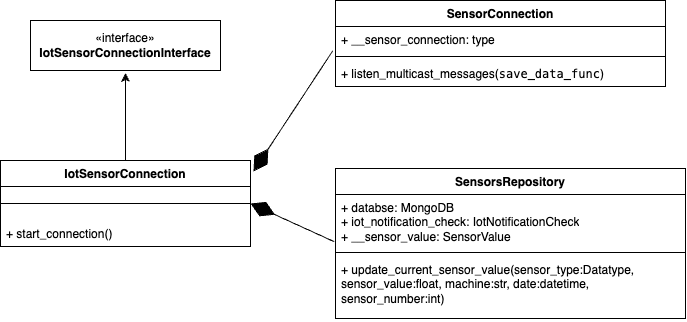
\includegraphics[width=\textwidth]{images/recebimento_dados.png}
	\caption{Module to receive sensor data.}
	\label{fig:receiveData}
\end{figure}


\subsection{Modulo de processamento}
O módulo de processamento de dados foi desenvolvido para garantir que os dados brutos coletados sejam processados, fornecendo a análise estatística que é exibida para os usuários.

O código é executado quando é invocada uma função específica encarregada de realizar uma série de operações. Primeiramente, uma lista é constituída contendo as coleções do banco de dados responsáveis pelo armazenamento tanto dos dados brutos quanto dos dados já processados. Simultaneamente, uma segunda lista é gerada, representando as máquinas que enviaram informações para o sistema.

Com essas listas em mãos, inicia-se um procedimento iterativo. Para cada máquina identificada, os dados disponíveis são lidos, submetidos a um processo de análise estatística, após o qual os resultados obtidos são registrados na coleção de dados processados. Essa análise estatística adota o método do Box Plot.

%TODO Referencia para um artigo explicando sobre boxPlot
O Box Plot, também conhecido como diagrama de caixa, é uma ferramenta gráfica utilizada para representar a variação de dados observados de uma variável numérica por meio de quartis. Na figura ~\ref{fig:boxplot}, pode ser visto o retângulo formado pelo primeiro quartil (Q1), mediana e terceiro quartil (Q3), que fornecem uma noção sobre a centralidade e dispersão dos dados, enquanto as "antenas" estendem-se para mostrar a amplitude completa dos dados, ajudando assim na identificação de possíveis outliers.

Ao adotar o Box Plot, o sistema garante uma compreensão robusta da distribuição dos dados, identificando não apenas tendências centrais, mas também variações e potenciais anomalias.

\begin{figure}[htbp]
	\centering
	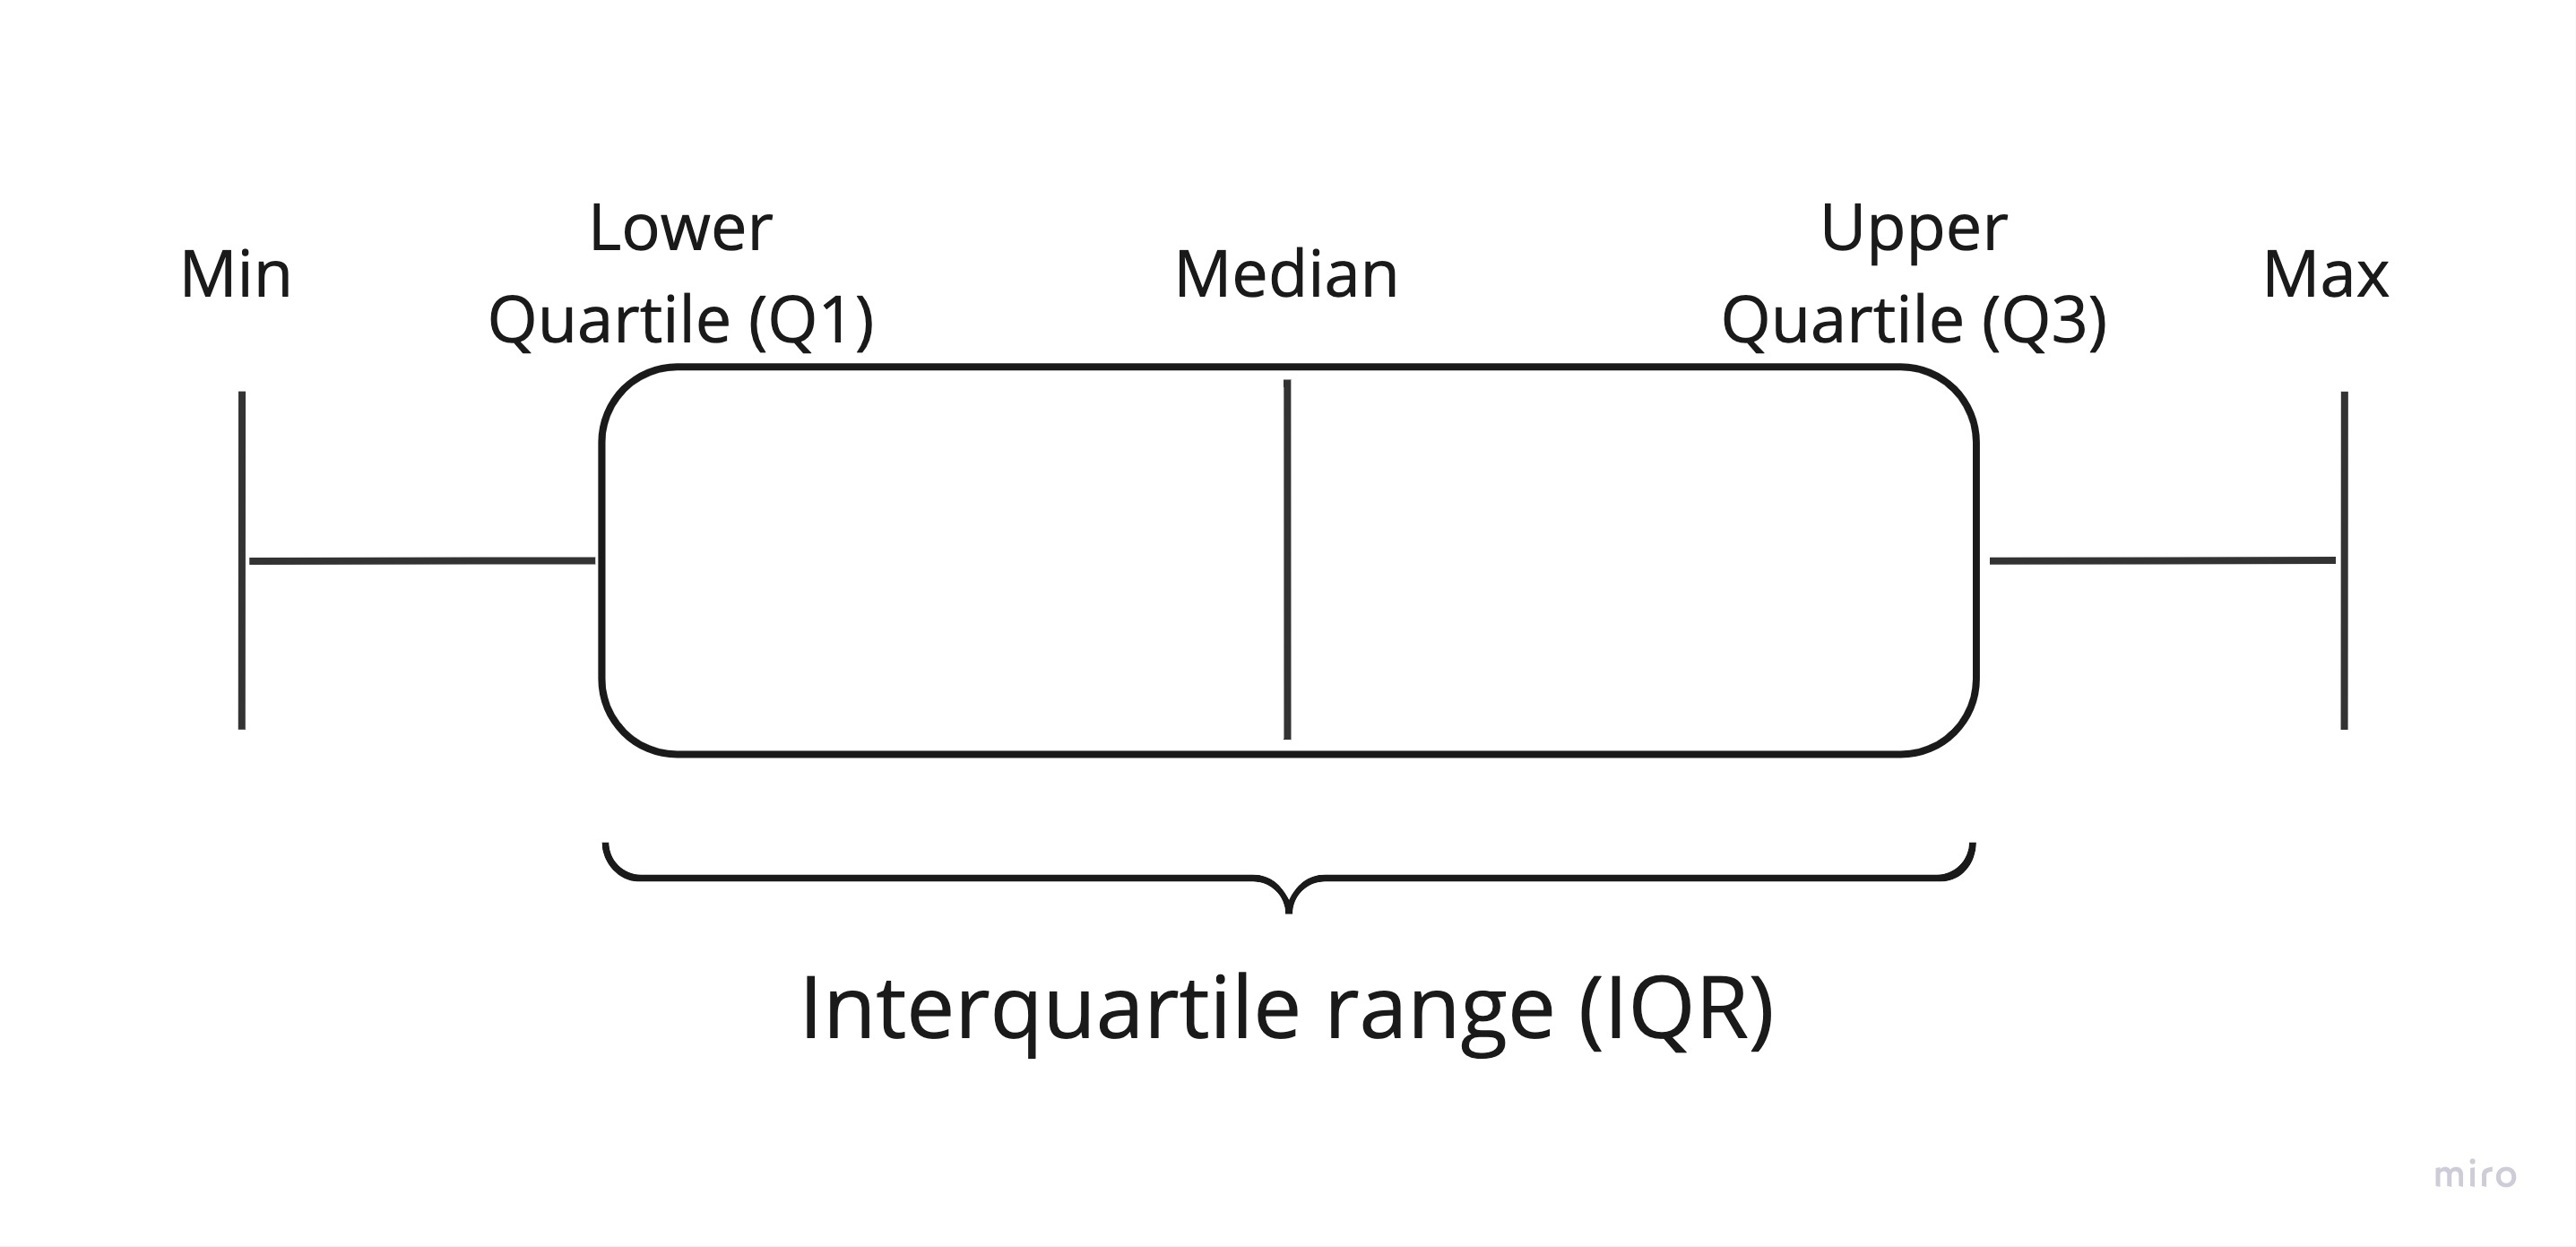
\includegraphics[width=\textwidth]{images/boxplot.jpg}
	\caption{BoxPlot.}
	\label{fig:boxplot}
\end{figure}


\subsection{API}
A API foi estruturada em pequenos sub-módulos, cada um focado em um contexto específico. Esta modularização assegura que cada parte da API tenha uma única responsabilidade. Em cada módulo, há uma segmentação composta por: a camada de \textit{controller}, destinada a receber e gerenciar as requisições HTTP; a camada de serviço, que serve para processar a informação e aplicar as respectivas regras de negócio; e a camada de repositório, cujo papel é estabelecer uma ponte com o banco de dados, acessando e disponibilizando os dados necessários. A figura ~\ref{fig:api_organization} representa a organização de pastas que foi utilizada para essa arquitetura.

\begin{figure}[htbp]
	\centering
	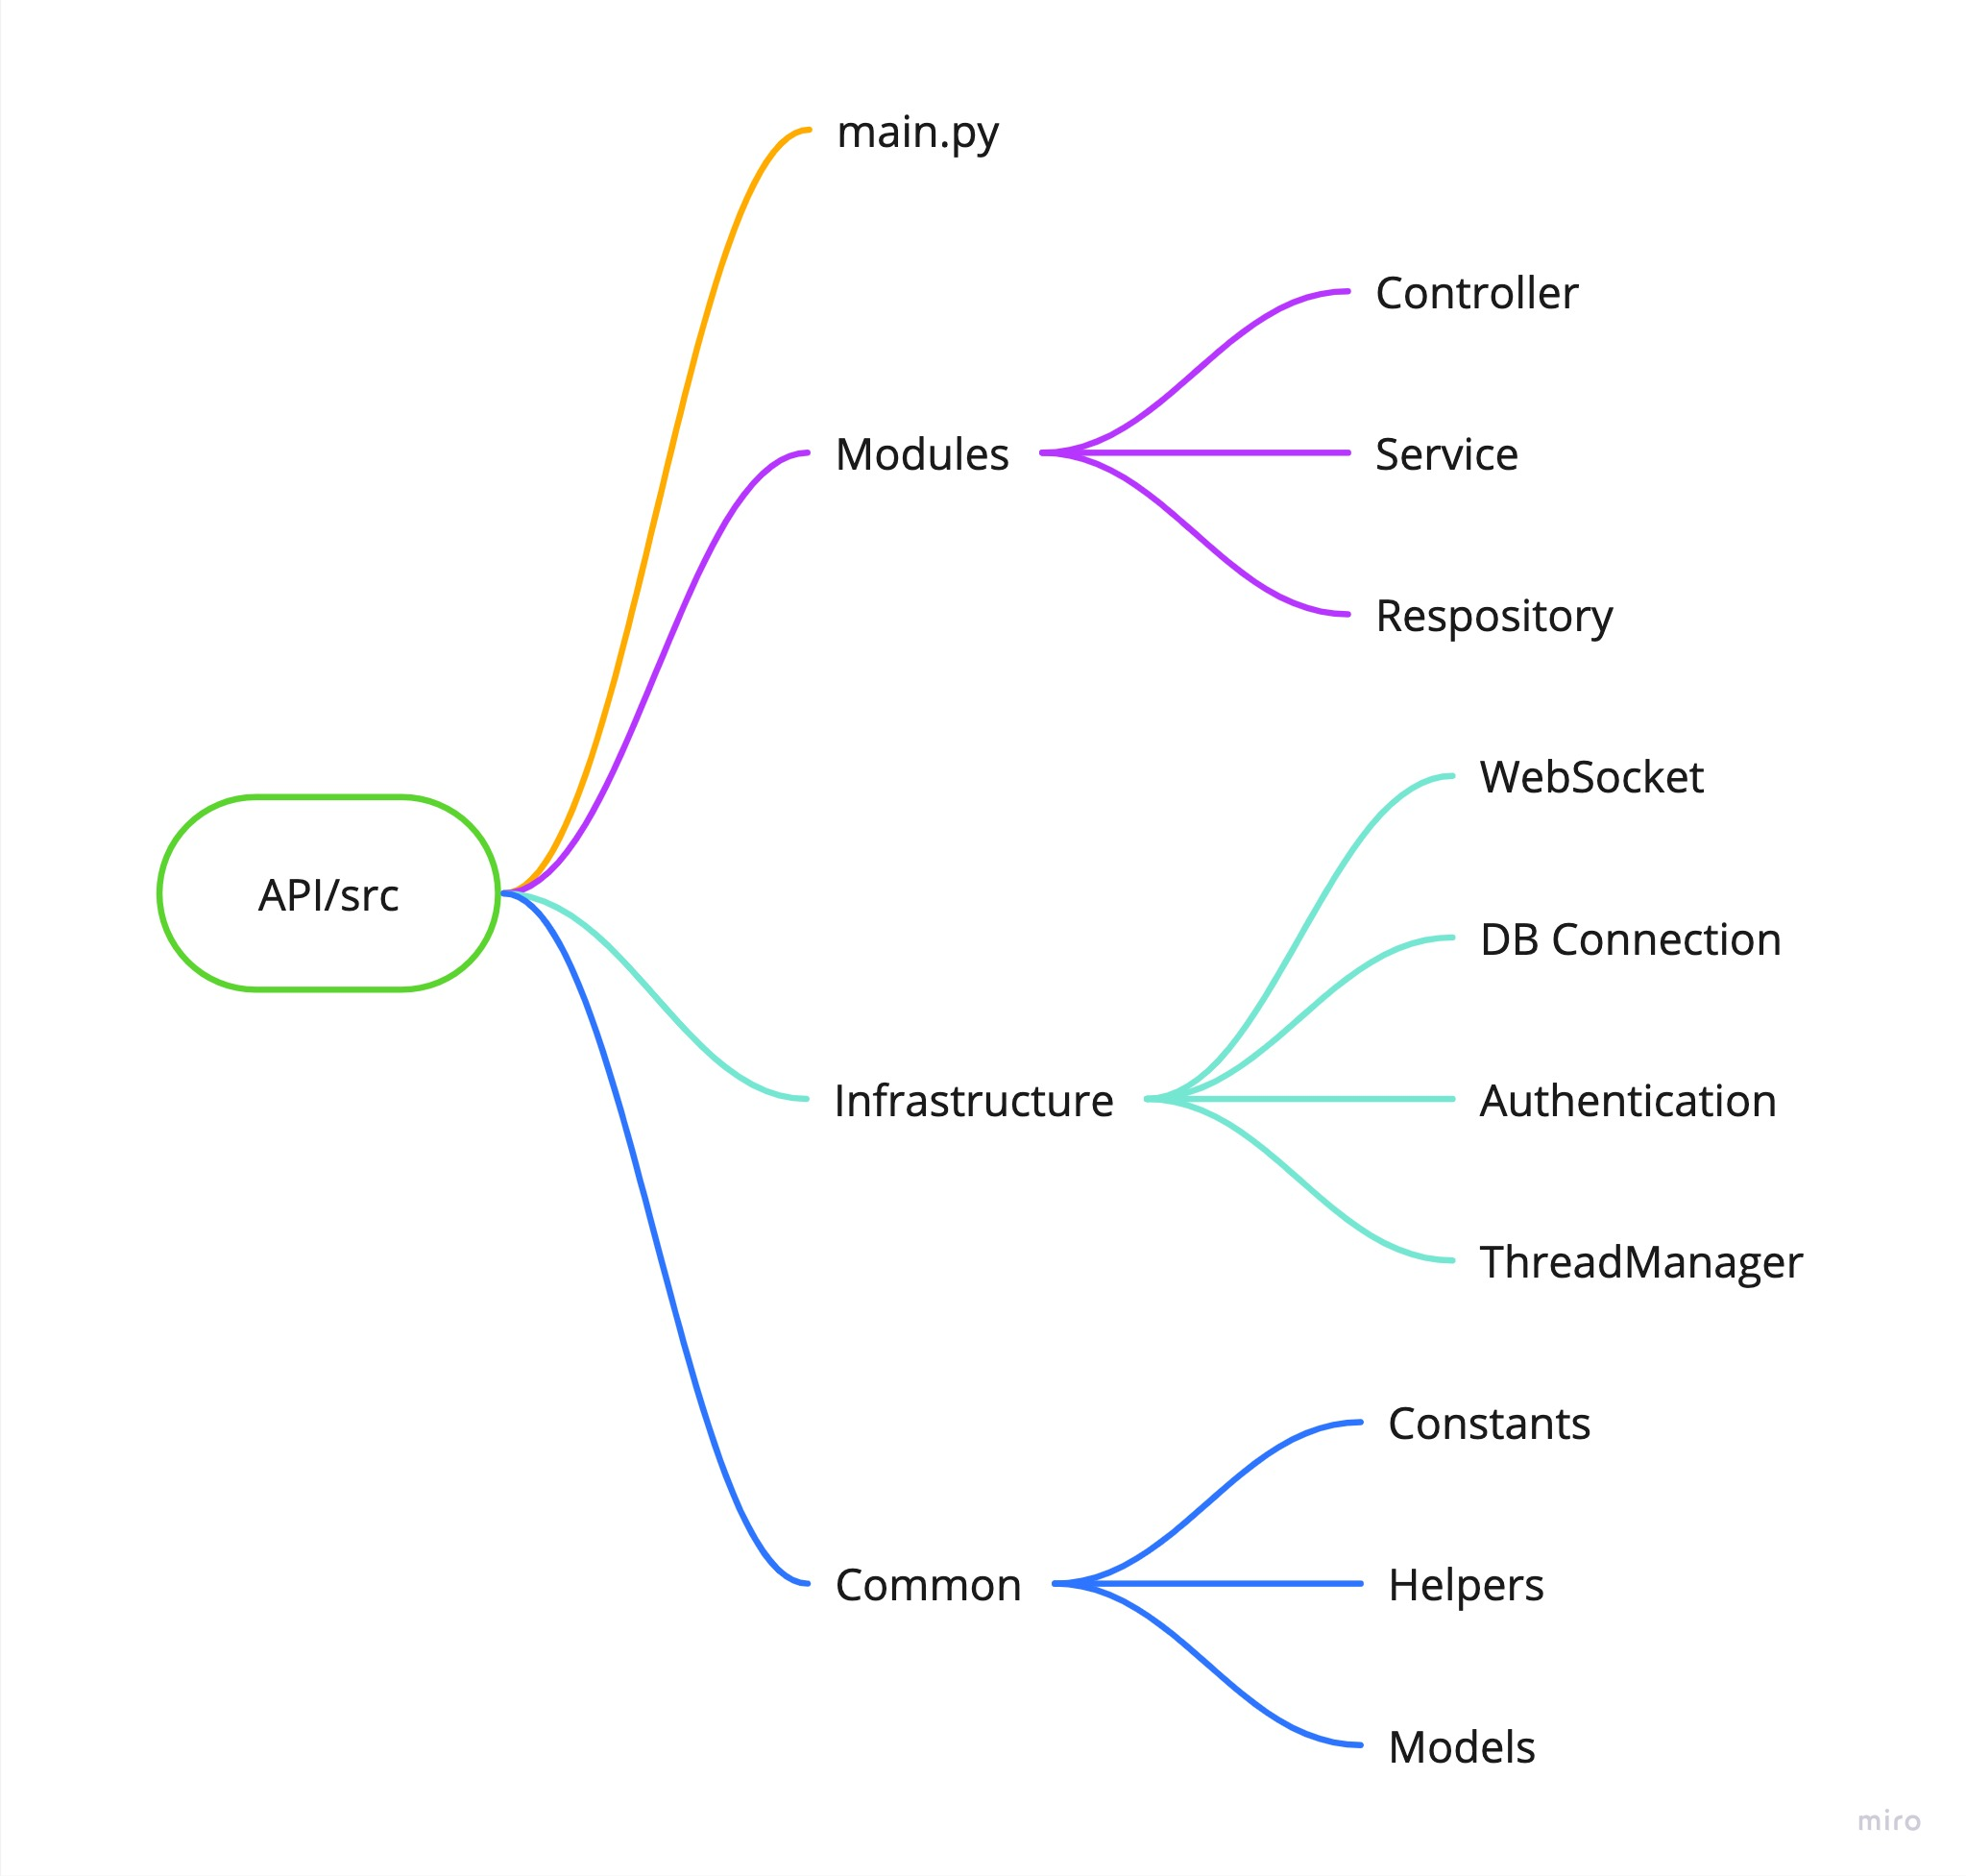
\includegraphics[width=\textwidth]{images/API_Organization.jpg}
	\caption{API Organization.}
	\label{fig:api_organization}
\end{figure}

Quando uma solicitação é enviada à API, a primeira interação acontece com a camada de \textit{controller}. Uma vez recebida, essa requisição é direcionada à camada de serviço, onde as regras de negócio são aplicadas. A camada de serviço se comunica estreitamente com a camada de repositório, que detém a responsabilidade de acessar o banco de dados e trazer informações precisas, adequadas às demandas do módulo em questão.

Os módulos implementados na API com a lógica descrita são:
\begin{itemize}
	\item \textbf{Downtime:} Responsável por gerenciar o acesso aos dados de paragem armazenados para teste no sistema.
	\item \textbf{IOT Sensors:} Responsável por gerenciar o acesso aos dados referentes aos sensores das maquinas na fabrica.
	\item \textbf{Notification:} Responsável por gerenciar o acesso as notificações geradas pelo sistema, e também as conexões web sockets para envio de notificações.
	\item \textbf{User:} Responsável por gerenciar o acesso aos dados dos usuários, assim como realizar as operações de login e logout. 
\end{itemize}

Além dessas camadas modulares, existe uma área especifica na API para o armazenamento de códigos comuns a todos os módulos. Esta seção engloba diversas funções úteis, modelos de classes, valores constantes e configurações padrão. Tais elementos garantem uma maior coesão e reduzem a repetição de código, otimizando o desempenho geral. Dentre as configurações padrão, merecem destaque o inicializador que estabelece o acesso ao banco de dados, middleware de autenticação, conexão web socket para envio de notificações, e o inicializador de novas \textit{threads}. Este último é utilizada para operações assíncronas que são executadas em paralelo a operação da API, como aquelas executadas pelo módulo de recebimento de dados.

\section[Arquitetura do frontend]{Arquitetura do frontend}
- Next JS e estrutura pre definida de pastas para as paginas do sistema
- Componentes e layouts
- Context API e seu uso
- Acesso a camada externa (API)

\section{Containers}
Explicar sobre os containers

\section{Web Server}
Explicar sobre o NGINX

\section[Princípios do SOLID]{Princípios do SOLID}
Tópicos explicando cada uma das letras do SOLID e relacionando com exemplos concretos do sistema